% VUT FIT 1MITAI
% TIN 2019/2020
% Project: Task 3
% Author: Vladimir Dusek, xdusek27
% Date: 27/12/2019
% File: xdusek27.tex

%%%%%%%%%%%%%%%%%%%%%%%%%%%%%%%%%%%%%%%%%%%%%%%%%%%%%%%%%%%%%%%%%%%%%

\documentclass[11pt, a4paper, titlepage]{article}
\usepackage[left=2cm, text={17cm, 24cm}, top=3cm]{geometry}
\usepackage[utf8]{inputenc}
\usepackage[czech]{babel}
\usepackage{pdfpages}
\usepackage{amssymb}
\usepackage{multicol}
\usepackage{enumitem}
\usepackage{amsmath}
\usepackage{scrextend}
\usepackage{float}

\newcommand{\N}{\mathbb{N}_0}

\setlength\parindent{0pt}

%%%%%%%%%%%%%%%%%%%%%%%%%%%%%%%%%%%%%%%%%%%%%%%%%%%%%%%%%%%%%%%%%%%%%

\begin{document}

\begin{titlepage}
    \begin{center}
        \begin{figure}[htb]
            \centering
            
\includegraphics[width=0.85\hsize]{images/fitlogo.pdf}
        \end{figure}
        \vspace{\stretch{0.382}}
        {\Huge Teoretická informatika} \\
        \bigskip
        {\LARGE Úkol 3} \\
        \vspace{\stretch{0.618}}
    \end{center}
    {\Large \today \hfill Vladimír Dušek, xdusek27}
\end{titlepage}

%%%%%%%%%%%%%%%%%%%%%%%%%%%%%%%%%%%%%%%%%%%%%%%%%%%%%%%%%%%%%%%%%%%%%

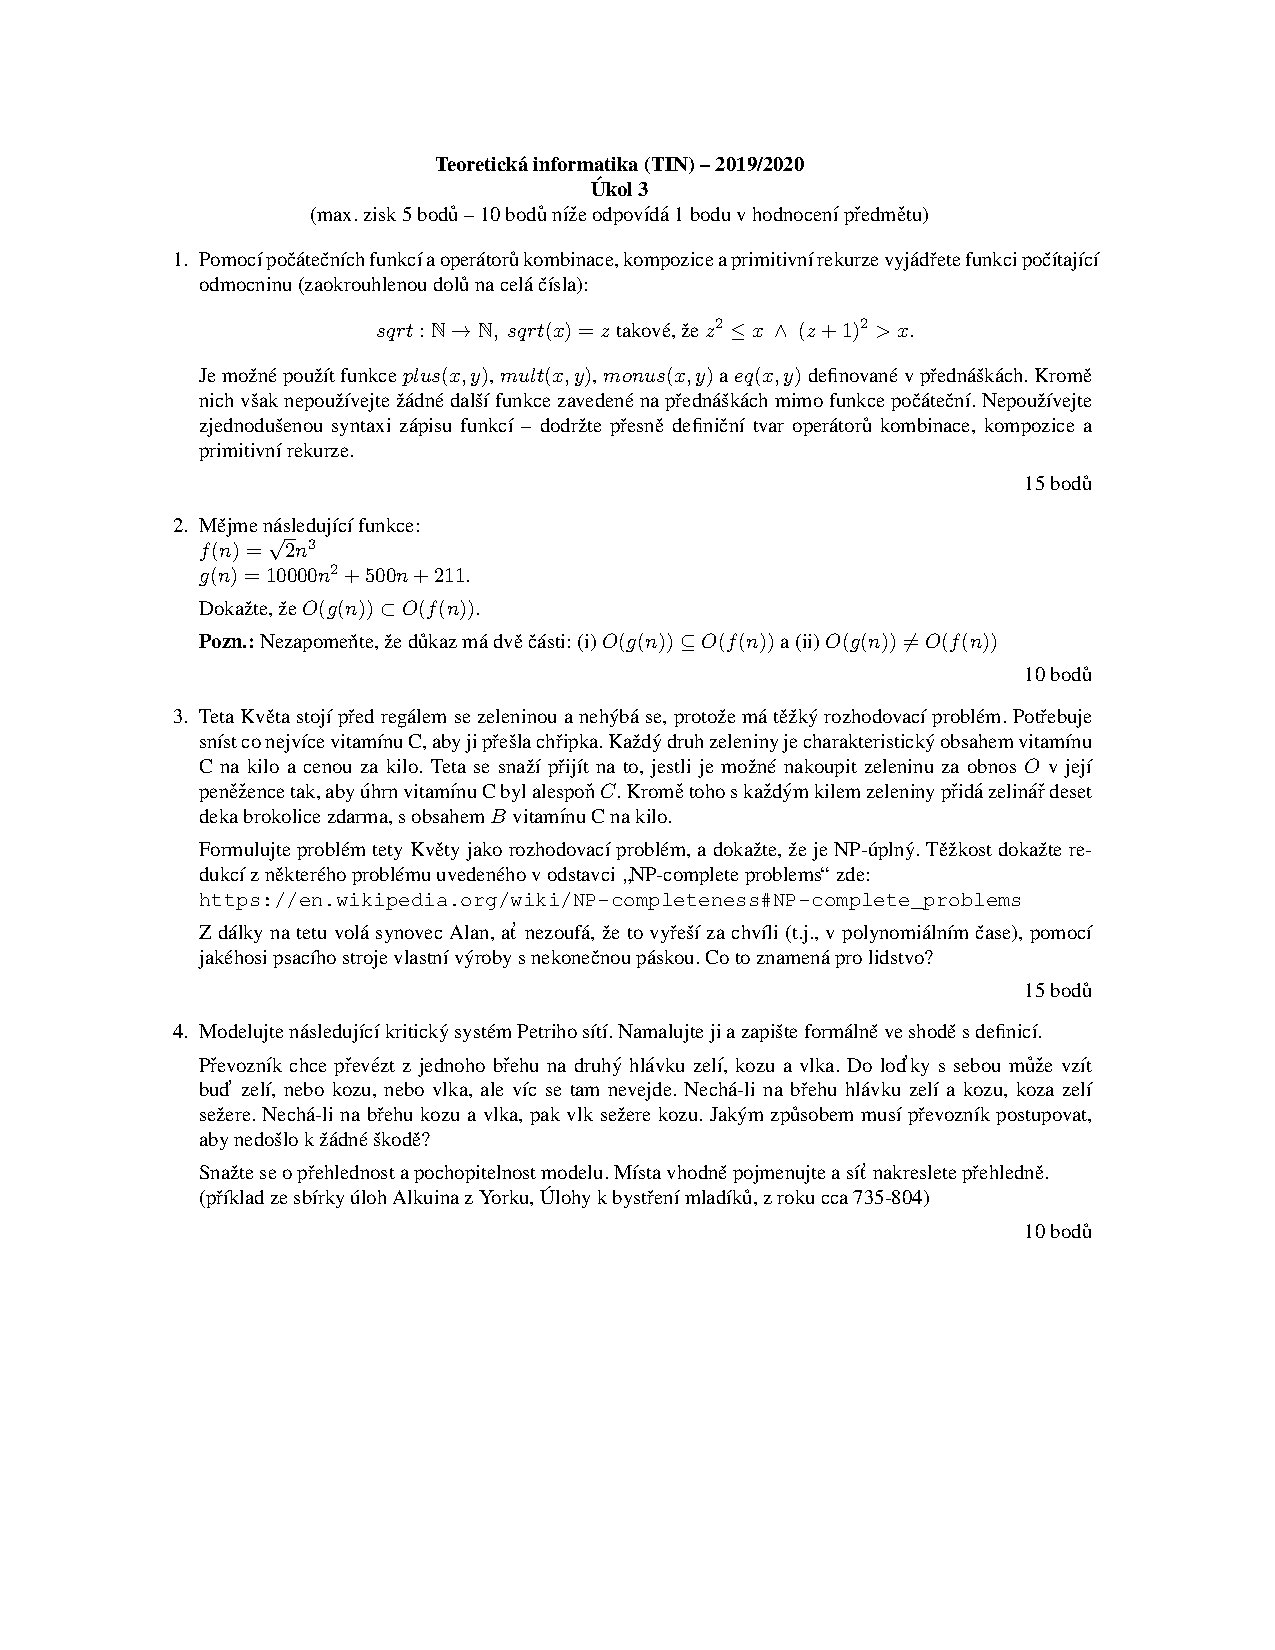
\includepdf{assignment.pdf}

%%%%%%%%%%%%%%%%%%%%%%%%%%%%%%%%%%%%%%%%%%%%%%%%%%%%%%%%%%%%%%%%%%%%%

\section*{Příklad 1}

% ToDo:
% - Nutne vice popsat a vysvetlit?
% - Napr. pomoci matematickeho vyjadreni funkci?

Použité funkce $plus(x, y)$, $monus(x, y)$, $mult(x, y)$ a $eq(x, y)$ odpovídají definicím z přednášek.
\bigskip

Pomocná funkce $neg(x)$:

\begin{itemize}
	\item $neg(x) = monus (\sigma \circ \xi(), x)$
\end{itemize}

Pomocná funkce $isGreater(x, y)$:

\begin{itemize}
	\item $isGreater(x, y) = neg \circ eq(monus(x, y), \xi())$
\end{itemize}

Pomocná funkce $foo(x, y)$:

\begin{itemize}
	\item $foo(0, y) = \xi()$
	\item $foo(x+1, y) = plus (isGreater (mult(\sigma \times \sigma(x)), y), foo(x, y))$
\end{itemize}

Výsledná funkce $sqrt(x)$:

\begin{itemize}
	\item $sqrt(x) = monus (x,  foo(x, x))$
\end{itemize}

\newpage

%%%%%%%%%%%%%%%%%%%%%%%%%%%%%%%%%%%%%%%%%%%%%%%%%%%%%%%%%%%%%%%%%%%%%

\section*{Příklad 2}

\begin{figure}[H]
	\begin{center}
		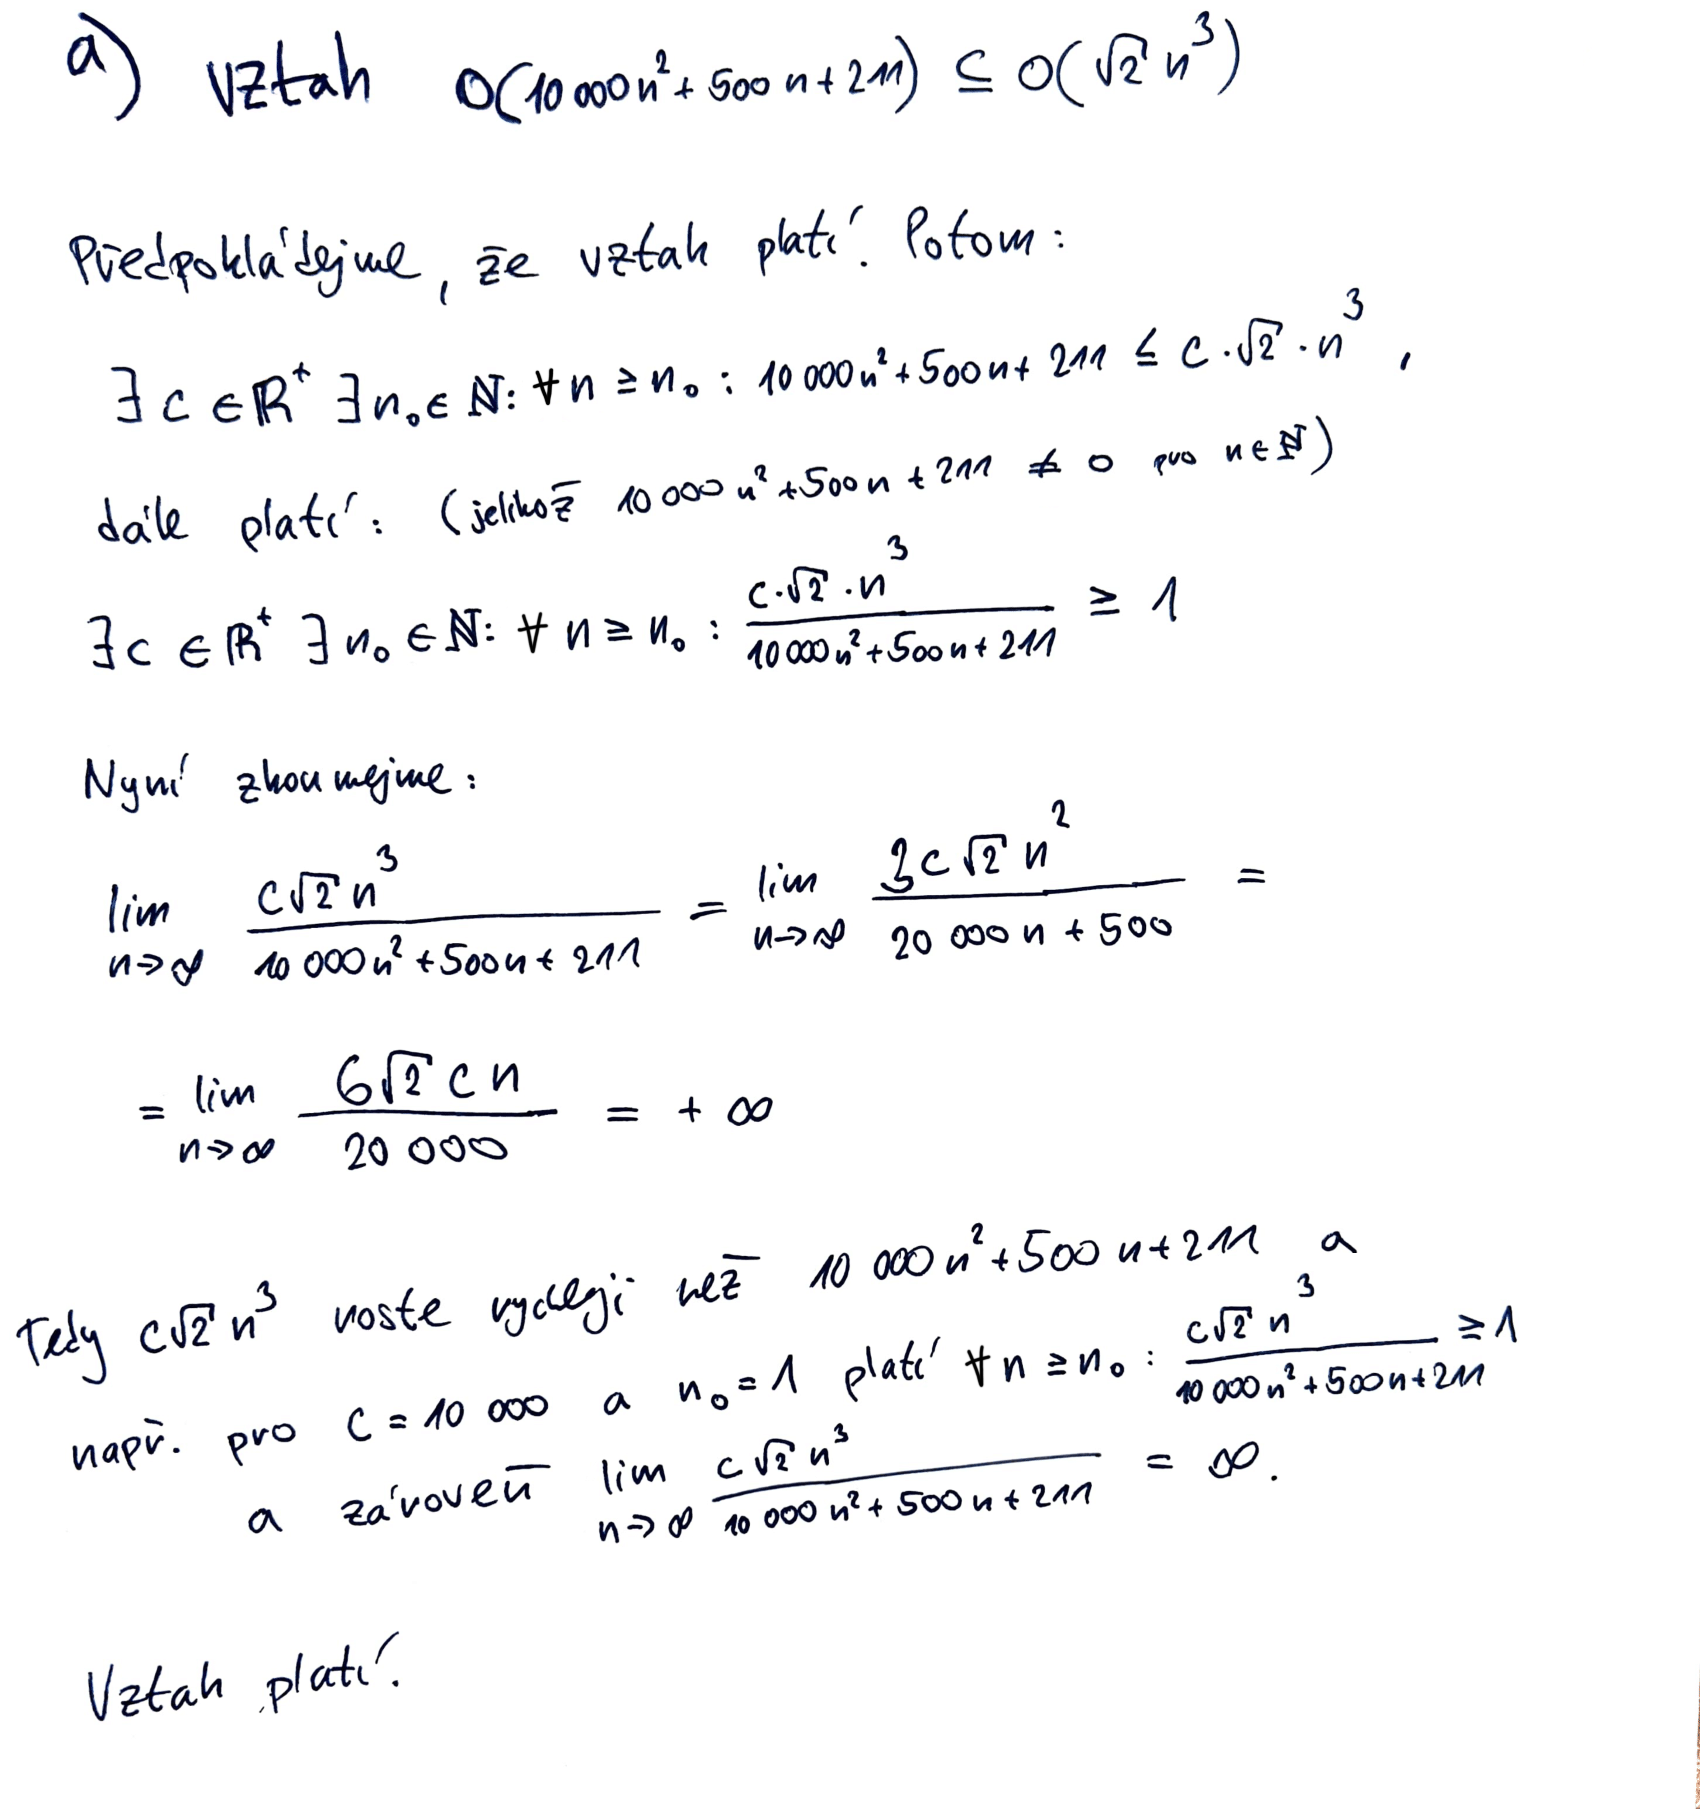
\includegraphics[page=1,scale=0.55]{images/tin-4-2-1.png}
	\end{center}
\end{figure}

\begin{figure}[H]
	\begin{center}
		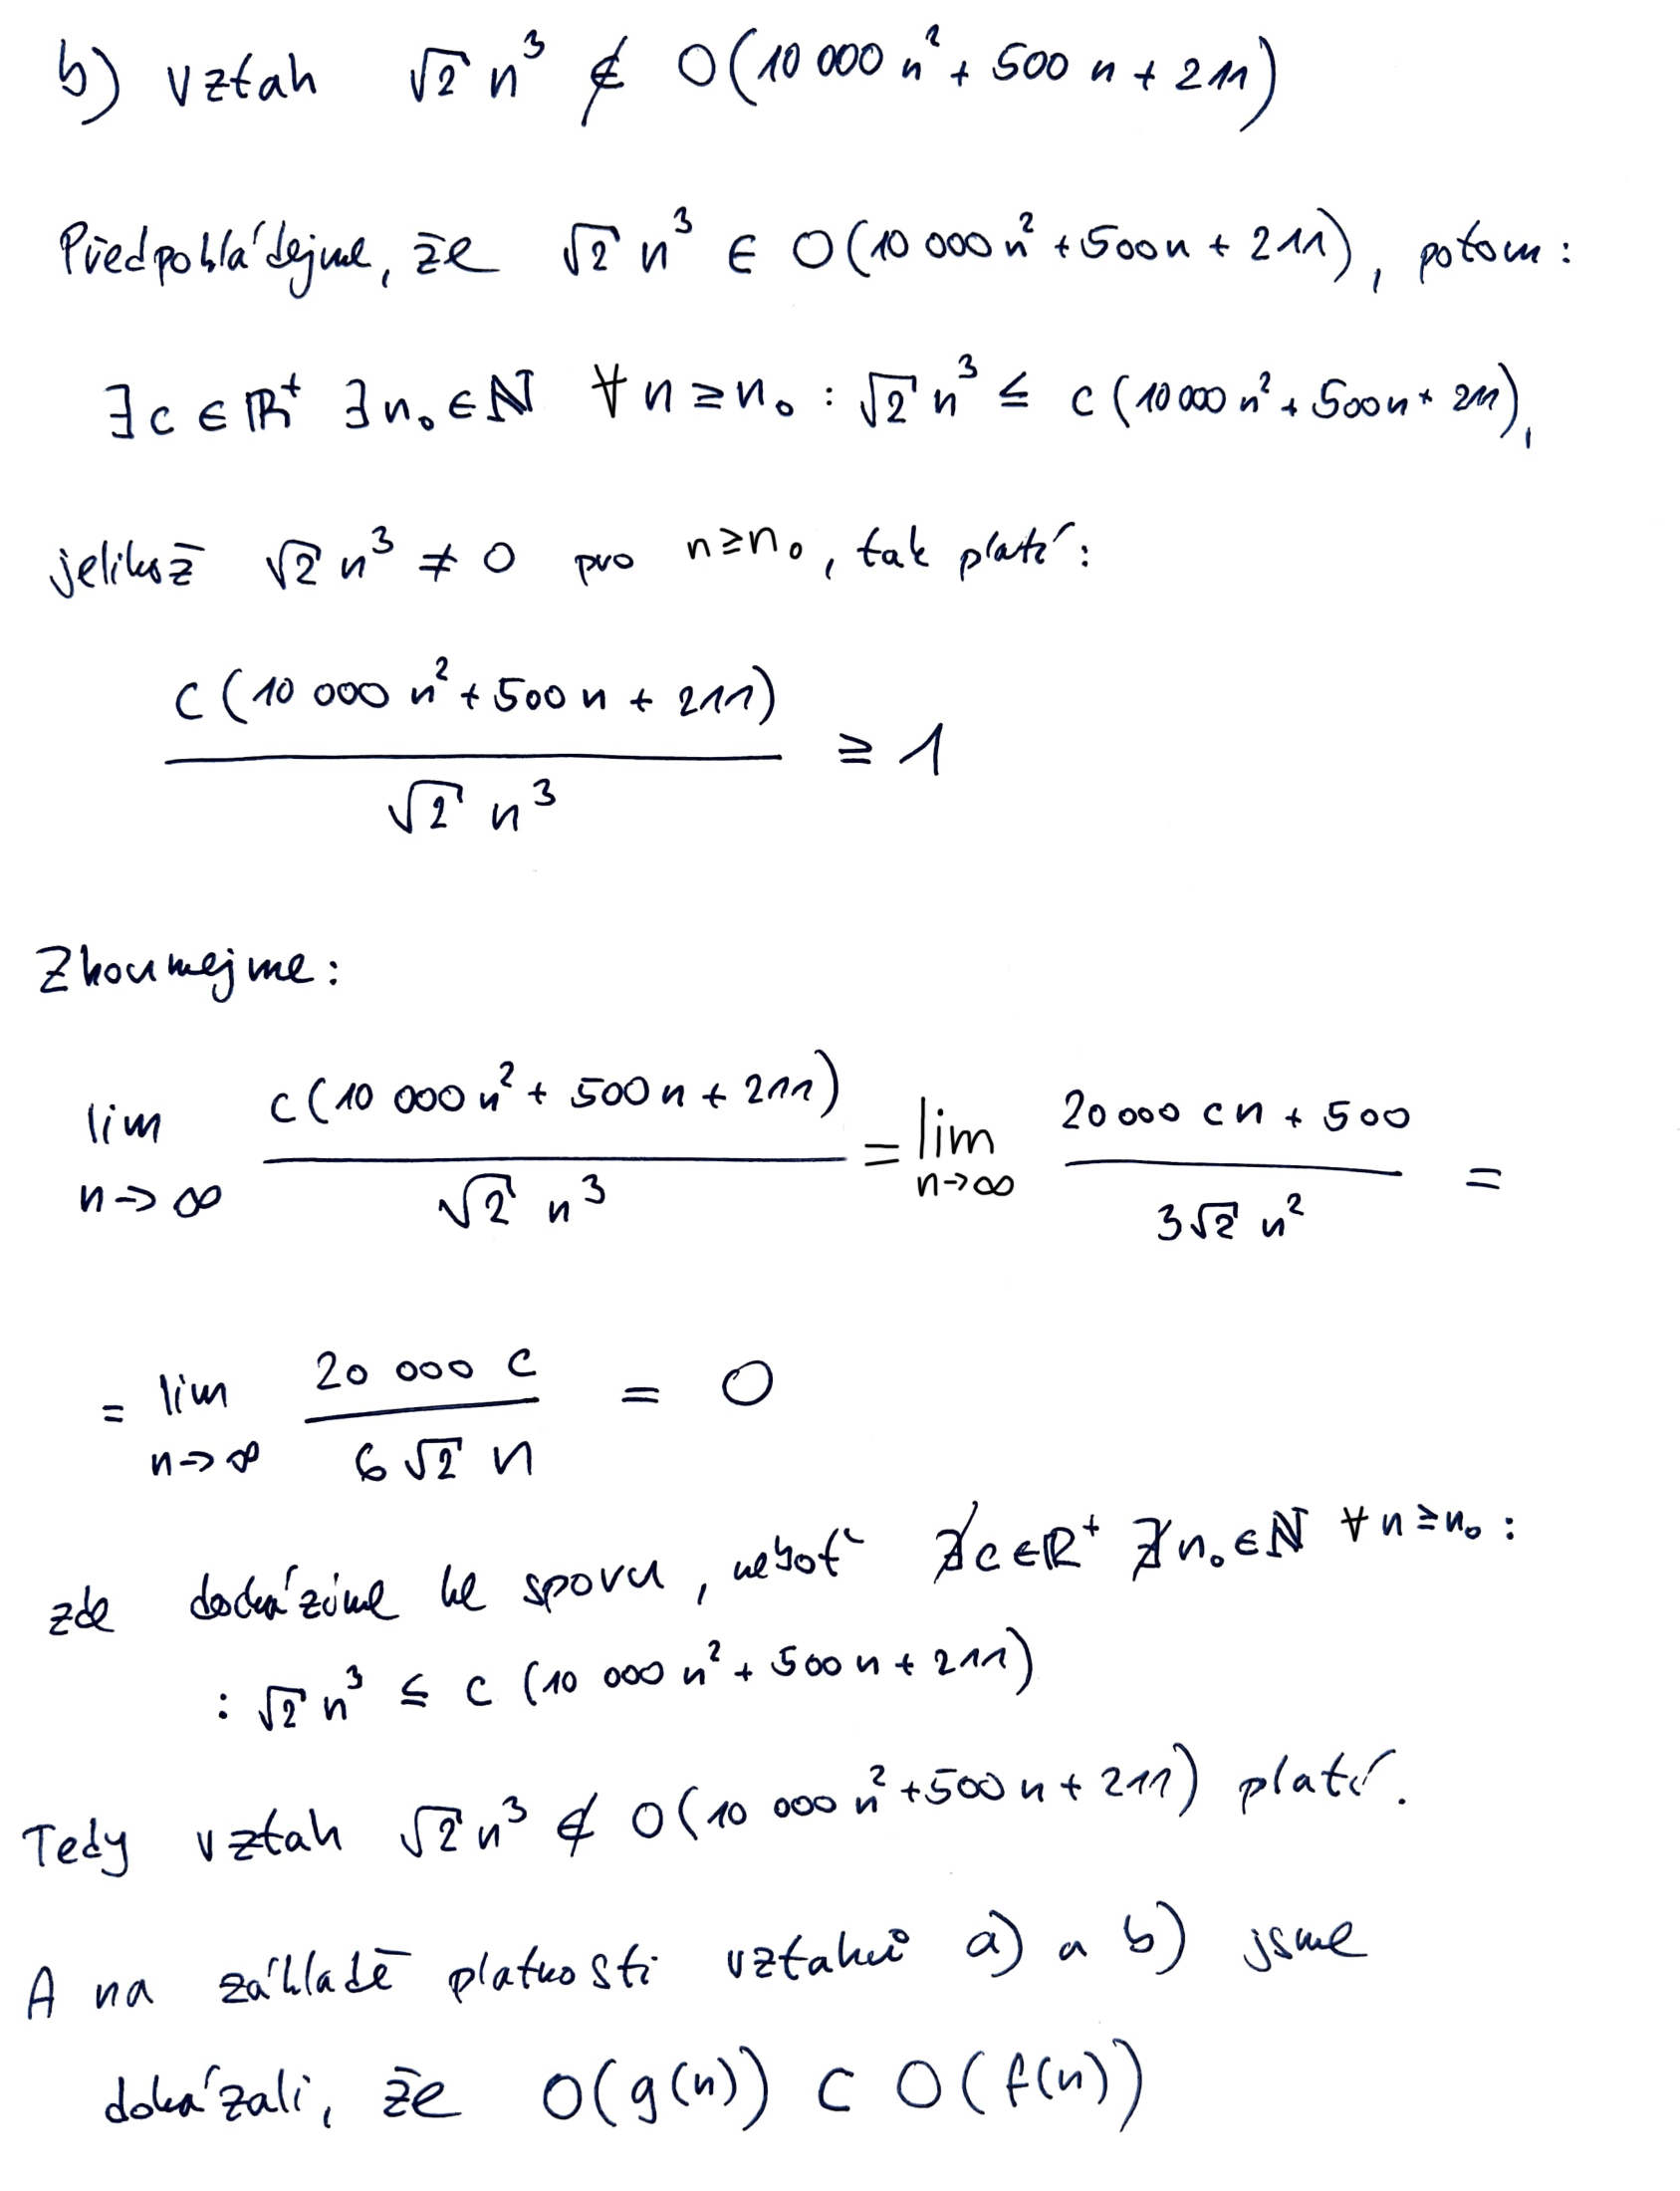
\includegraphics[page=1,scale=0.5]{images/tin-4-2-2.png}
	\end{center}
\end{figure}

\newpage

%%%%%%%%%%%%%%%%%%%%%%%%%%%%%%%%%%%%%%%%%%%%%%%%%%%%%%%%%%%%%%%%%%%%%

% \section*{Příklad 3}

% ToDo

% \newpage

%%%%%%%%%%%%%%%%%%%%%%%%%%%%%%%%%%%%%%%%%%%%%%%%%%%%%%%%%%%%%%%%%%%%%

\section*{Příklad 4}

Kritický systém Vlk, koza a zelí modeluje následující Petriho síť: $PN = (P, T, F, W, K, M_0)$, kde

\begin{itemize}[label=$\circ$]
	\item $P = \{ p_1, p_2, p_3, p_4, p_5, p_6, p_7, p_8, p_9, p_{10}, p_{11}, p_{12} \}$
	\item $T = \{ t_1, t_2, t_3, t_4, t_5, t_6, t_7, t_8, t_9, t_{10}, t_{11}, t_{12}, t_{13}, t_{14} \}$
	\item $F = \{ (p_1, t_1), (p_1, t_5), (p_2, t_2), (p_2, t_5), (p_2, t_6), (p_3, t_3), (p_3, t_6), (p_4, t_1), (p_4, t_2), (p_4, t_3), (p_4, t_13), (p_5, t_5),$

	$(p_5, t_6), (p_5, t_14), (p_6, t_4), (p_7, t_7), (p_7, t_{11}), (p_8, t_8), (p_8, t_{11}), (p_8, t_{12}), (p_9, t_9), (p_9, t_{12}), (p_{10}, t_{7}), (p_{10}, t_{8}),$

	$(p_{10}, t_{9}), (p_10, t_14), (p_{11}, t_{11}), (p_{11}, t_{12}), (p_{11}, t_{10}), (p_11, t_13), (p_{12}, t_{10}), (t_{1}, p_{12}), (t_{1}, p_{7}), (t_{1}, p_{5}), (t_{2}, p_{12}),$

	$(t_{2}, p_{8}), (t_{2}, p_{5}), (t_{3}, p_{12}), (t_{3}, (p_{9}), (t_{3}, p_{5}), (t_{4}, p_{4}), (t_{5}, p_{2}), (t_{5}, p_{5}), (t_{6}, p_{3}), (t_{6}, p_{5}), (t_{7}, p_{1}), (t_{7}, p_{6}),$

	$(t_{7}, p_{11}), (t_{8}, p_{2}), (t_{8}, p_{6}), (t_{8}, p_{11}), (t_{9}, p_{3}), (t_{9}, p_{6}), (t_{9}, p_{11}), (t_{10}, p_{10}), (t_{11}, p_{8}), (t_{11}, p_{11}), (t_{12}, p_{9}),$

	$(t_{12}, p_{11}), (t_{13}, p_{10}), (t_{14}, p_{4}) \}$

	\item $W = \{ (f, 1) \mid f \in F \}$

	\item $K = \{ (p, 1) \mid p \in P \}$

	\item $M_0 = \{ (p_1, 1), (p_2, 1), (p_3, 1), (p_4, 1), (p_5, 0), (p_6, 0), (p_7, 0), (p_8, 0), (p_9, 0), (p_{10}, 0), (p_{11}, 1), (p_{12}, 0) \}$
\end{itemize}

Nákres Petriho sítě $PN$ je na obrázku~\ref{petri-net}.

\begin{figure}[H]
	\begin{center}
		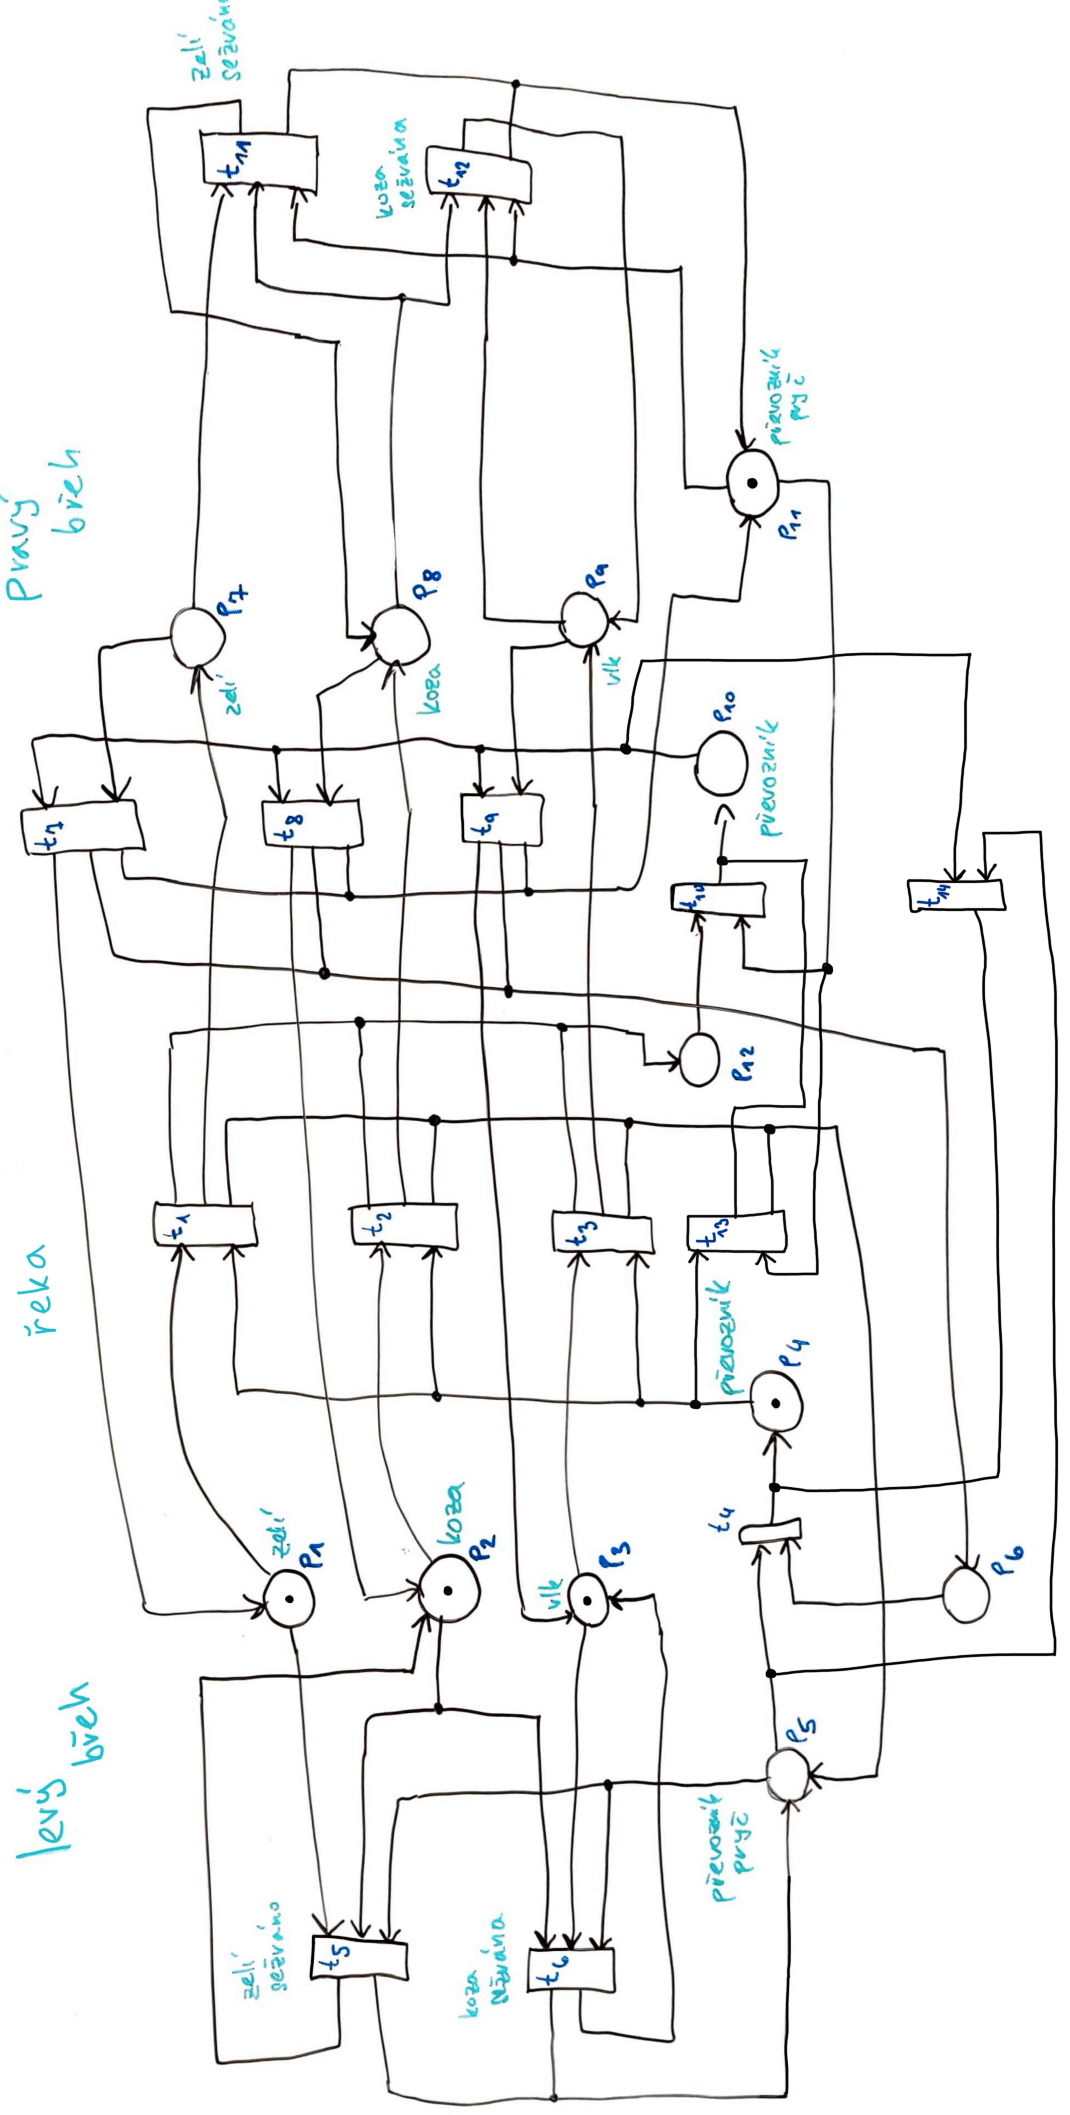
\includegraphics[page=1,scale=0.3]{images/petri-net-fix-rotated.png}
		\caption{Petriho síť modelující systém Vlk, koza a zelí.}
		\label{petri-net}
	\end{center}
\end{figure}

\newpage

%%%%%%%%%%%%%%%%%%%%%%%%%%%%%%%%%%%%%%%%%%%%%%%%%%%%%%%%%%%%%%%%%%%%%

\end{document}
